\documentclass[12pt]{article}
\usepackage[a4paper,%bindingoffset=0.2in,%
            left=2cm,right=2cm,top=2.5cm,bottom=2.5cm,%
            footskip=1.2cm]{geometry}
%\textwidth 15.5cm \oddsidemargin 0.4cm 
%\topmargin -1cm

%\textheight 24cm 
\footskip 1cm 
\usepackage{epsfig}
\usepackage{amsmath,graphicx,psfrag,pstcol,caption}
\usepackage{float}
\usepackage{amsfonts}
\usepackage{mathtools}
\usepackage{gensymb}
\usepackage{textgreek}
\usepackage{afterpage,natbib,lipsum}
\usepackage{subcaption}
\usepackage{bm}
\def\n{\noindent}
\def\u{\underline}
\def\hs{\hspace}
\newcommand{\thrfor}{.^{\displaystyle .} .}
\newcommand{\bvec}[1]{{\bf #1}}
\setlength{\parindent}{0ex}
\setlength{\abovecaptionskip}{0pt}
\setlength{\belowcaptionskip}{-10pt}

\begin{document}

\noindent
\rule{17.0cm}{0.5mm}
\vspace{0.7cm}


Engineering Tripos Part IIB \hfill F-YA331-1

\begin{center}
{\large{\bf Complex Biological Synapses for Unsupervised Learning in Non-Stationary Environments}}\\
\vspace{1mm}
{\bf Summary on Preparatory Work}\\
\vspace{2mm}
Name: Yuhao Wang\\
College: Peterhouse\\
CRSid: yw451
\end{center}
\rule{17cm}{0.5mm}

% \vspace*{1cm}
% \begin{center}
% \fbox{\parbox{0.8\linewidth}{\bf This  is a template suitable for the short report write-up. Simply edit the Latex or Word document to include your calculations/ results/ code.}}
% \end{center}
% \vspace*{1cm}

\section{Learning Rule}

The learning rule used here is the Oja (1982) rule, which is a Hebbian rule with dynamic constraint. It can be expressed as
\begin{equation}
    \tau_w \dfrac{d\boldsymbol{w}}{dt} = v\boldsymbol{u} - \alpha v^2 \boldsymbol{w},
\end{equation}
where $\tau_w$ is a time constant, $\boldsymbol{u}$ and $v$ are inputs and output of the neuron, respectively, $\boldsymbol{w}$ is the input synapse weight vector, and $\alpha$ is a positive constant. It can be shown that with this learning rule, $|\boldsymbol{w}|$ over time will relax to the value $1/\alpha$. $\boldsymbol{u}$ and $\boldsymbol{w}$ are $N$ dimensional vectors where $N$ is the number of input synapses connected to the neuron.

\section{Input Statistics}
The input vector at each moment is generated by sampling a random vector with multivariate Gaussian distribution $\mathcal{N}(\boldsymbol{\mu}, \boldsymbol{C})$. For the time being $\boldsymbol{\mu}$ is kept at $\boldsymbol{0}$. $\boldsymbol{C}$ is constructed using

\begin{equation}
    \boldsymbol{C} = \boldsymbol{e}_1^T \boldsymbol{e}_1 + a\boldsymbol{I},
\end{equation}

with $\boldsymbol{e}_1$ being some arbitrary unit (not necessary but for convenience) $N$-dimensional vector, $a$ some constant and $\boldsymbol{I}$ the $N \times N$ identity matrix. 

\section{Results and Discussion}

\begin{figure}[ht]
  \centering
  \captionsetup{width = \textwidth}
  \begin{subfigure}[b]{0.32\textwidth}
    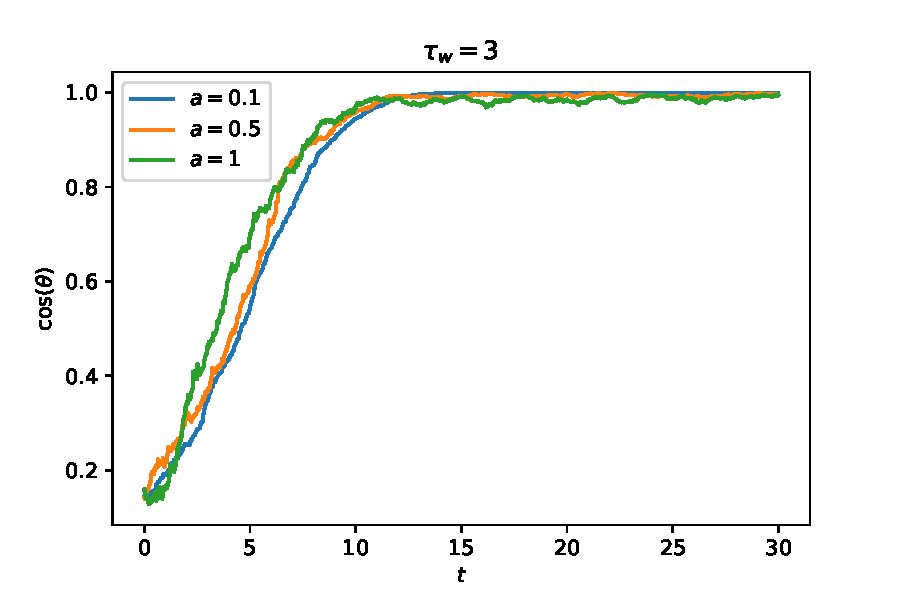
\includegraphics[width=\textwidth]{1.3.pdf}
    \caption{}
    \label{fig:1}
  \end{subfigure}
  %
  \begin{subfigure}[b]{0.32\textwidth}
    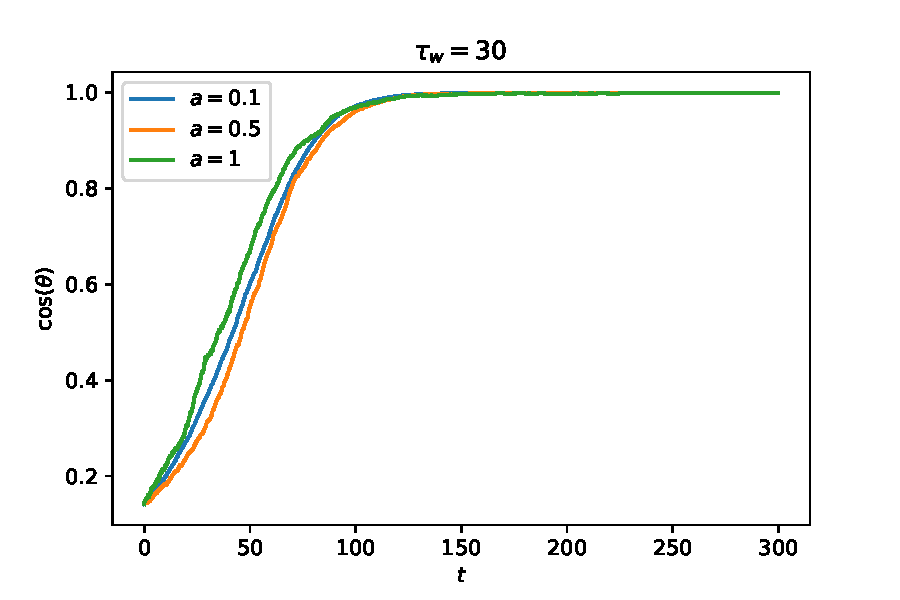
\includegraphics[width=\textwidth]{1.30.pdf}
    \caption{}
    \label{fig:2}
  \end{subfigure}
  %
  \begin{subfigure}[b]{0.32\textwidth}
    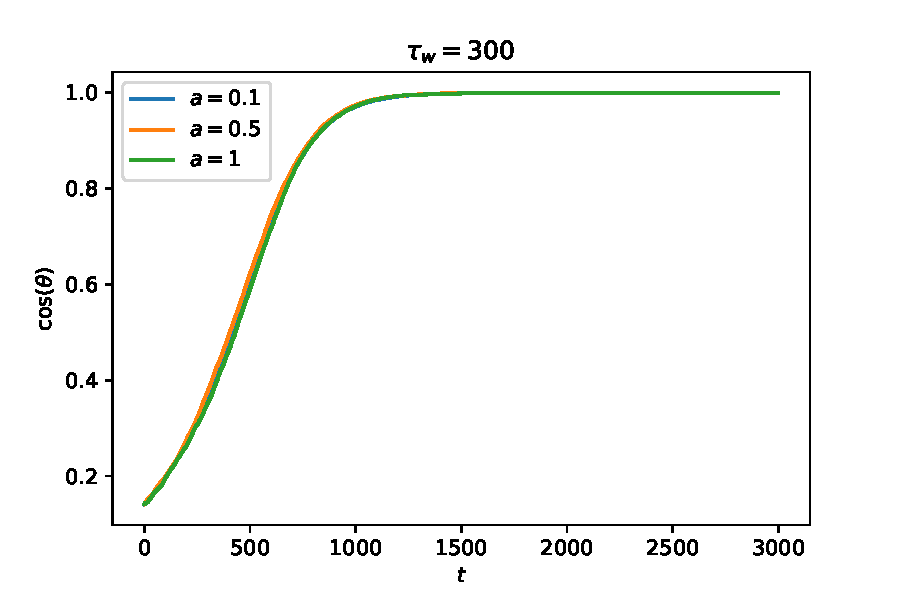
\includegraphics[width=\textwidth]{1.300.pdf}
    \caption{}
    \label{fig:3}
  \end{subfigure}  
  
  \vspace{0.6cm}
  
  \caption{}
  
\end{figure}

\begin{figure}[ht]
  \centering
  \captionsetup{width = \textwidth}
  \begin{subfigure}[b]{0.32\textwidth}
    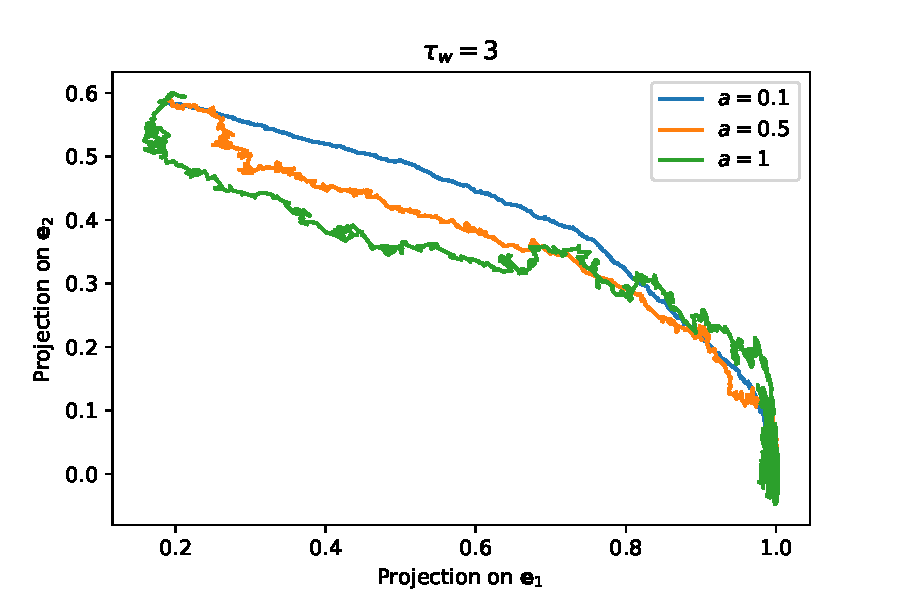
\includegraphics[width=\textwidth]{2.3.pdf}
    \caption{}
    \label{fig:1}
  \end{subfigure}
  %
  \begin{subfigure}[b]{0.32\textwidth}
    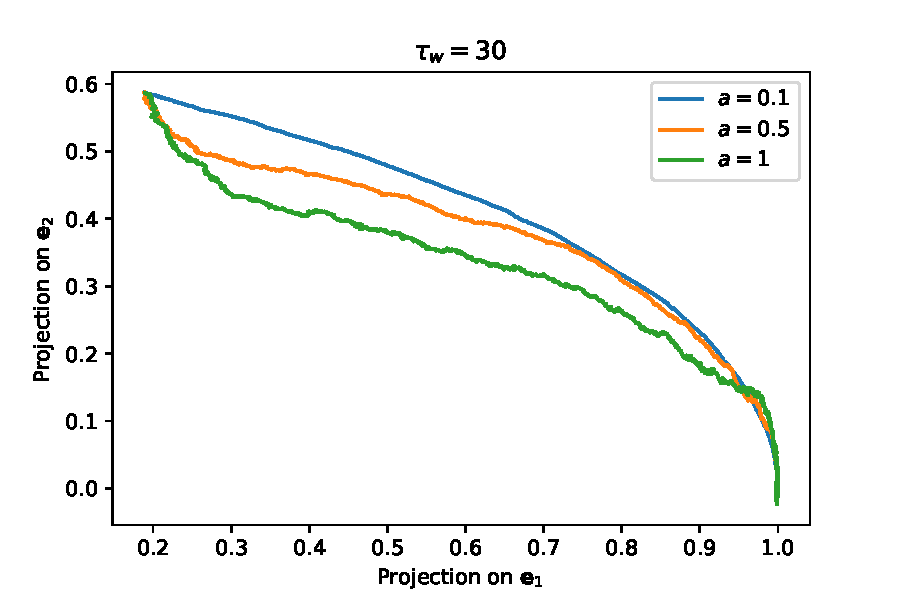
\includegraphics[width=\textwidth]{2.30.pdf}
    \caption{}
    \label{fig:2}
  \end{subfigure}
  %
  \begin{subfigure}[b]{0.32\textwidth}
    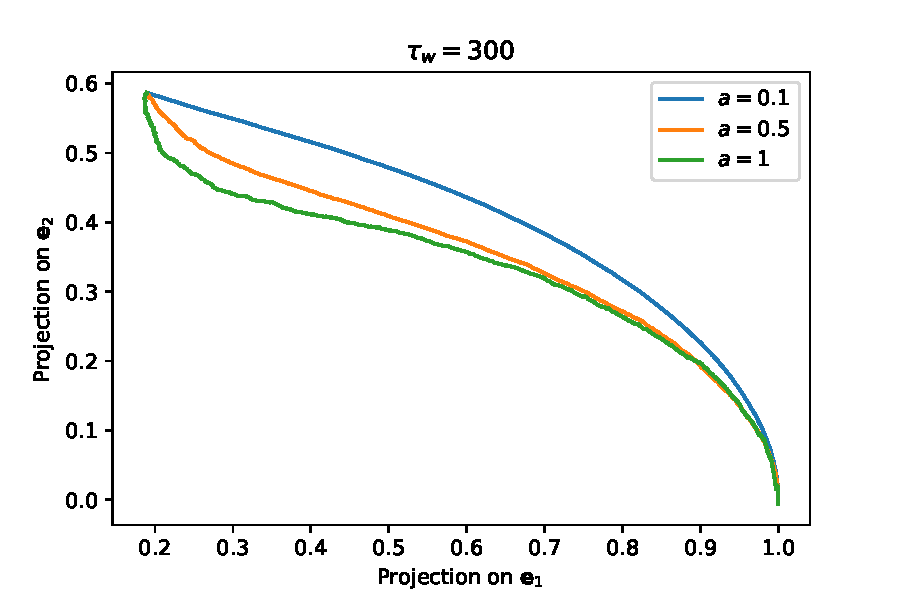
\includegraphics[width=\textwidth]{2.300.pdf}
    \caption{}
    \label{fig:3}
  \end{subfigure}  
  
  \vspace{0.6cm}
  
  \caption{}
  
\end{figure}

Figure 1 are plots of $\cos(\theta)$ against time, where $\theta$ is the angle between $\boldsymbol{w}$ and $\boldsymbol{e}_1$. Figure 2 are traces of $\boldsymbol{w}^T\boldsymbol{e}_1/|\boldsymbol{e}_1|$ plotted against $\boldsymbol{w}^T\boldsymbol{e}_2/|\boldsymbol{e}_2|$, where $\boldsymbol{e}_2$ is some arbitrary unit vector orthogonal to $\boldsymbol{e}_1$.  Note that to generate each of these plots, $\boldsymbol{w}$ is started from the same initial condition at $t=0$ and the input statistics is also kept constant both throughout each trial and across different trials. $\alpha = 1$ throughout the experiment.\\

As predicted by theoretical analysis (see Dayan and Abbott), these figures show that the direction of $\mathbb{E}\{\boldsymbol{w}(t)\} $ approaches that of $\boldsymbol{e}_1$ as $t \rightarrow \infty$. $\tau_w$ dominantly influences the speed of convergence (note the different scaling of time axes in Figure 1). $a$ influences the variance of $\boldsymbol{w}$, as it changes the relative magnitude of eigenvalues of other eigenvectors compared to the eigenvalue of $\boldsymbol{e}_1$. To be specific, $\lambda_1 = 1 + a$, $\lambda_2 = \dots = \lambda_N = a$. For the same $\tau_w$, larger values of $a$ gives greater variance.\\

$\tau_w$ also affects variance, as a slower dynamics more effectively filters out the higher frequency features of the input. The larger $\tau_w$ is, the more similar is the neuron's response to that generated by an averaged learning rule.

\begin{figure}[ht]
  \centering
  \captionsetup{width = \textwidth}
  \begin{subfigure}[b]{0.32\textwidth}
    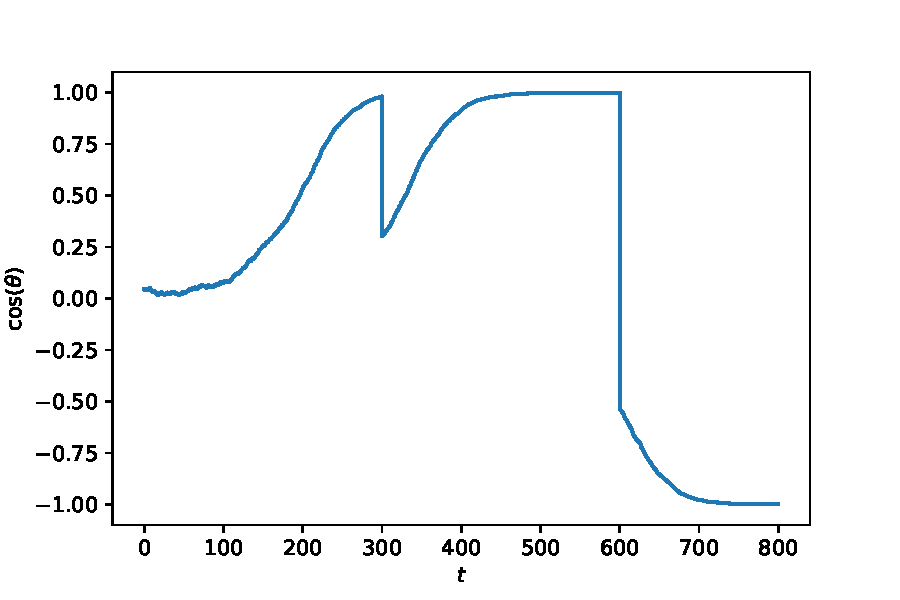
\includegraphics[width=\textwidth]{4.1.pdf}
    \caption{}
    \label{fig:1}
  \end{subfigure}
  %
  \begin{subfigure}[b]{0.32\textwidth}
    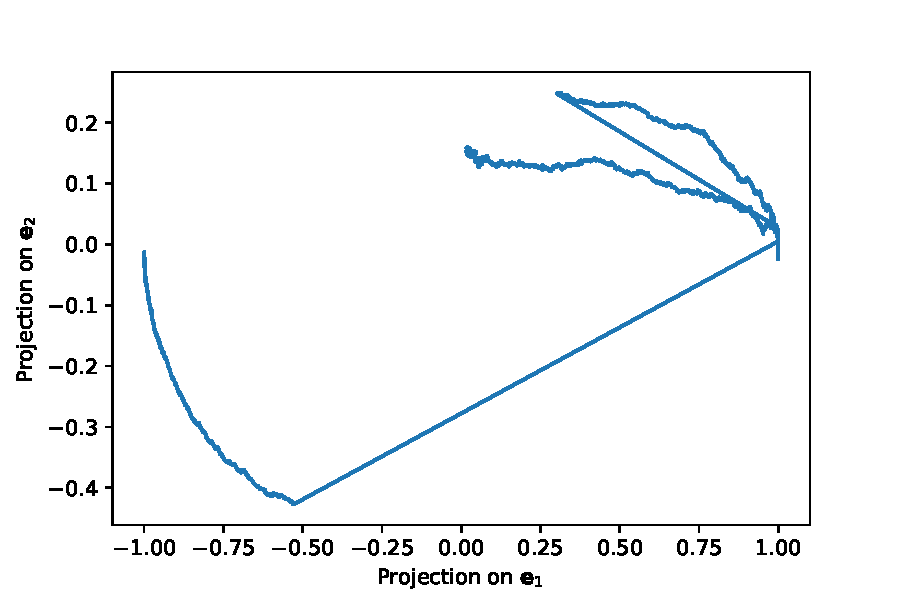
\includegraphics[width=\textwidth]{4.2.pdf}
    \caption{}
    \label{fig:2}
  \end{subfigure}
  %
  \begin{subfigure}[b]{0.32\textwidth}
    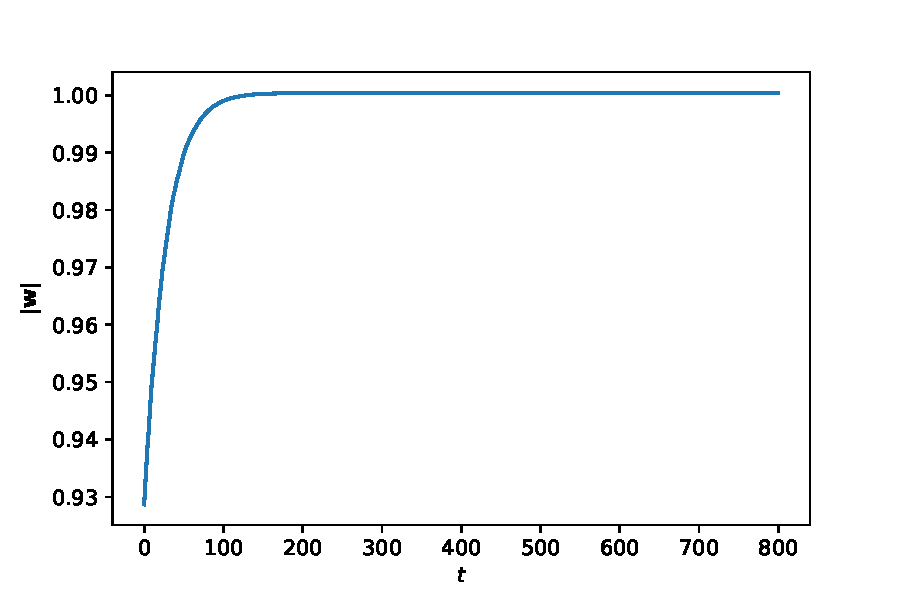
\includegraphics[width=\textwidth]{4.3.pdf}
    \caption{}
    \label{fig:3}
  \end{subfigure}  
  
  \vspace{0.6cm}
  
  \caption{}
  
\end{figure}

In the trial shown in Figure 3, $\boldsymbol{C}$ is no longer kept constant throughout the trial -- $\boldsymbol{e}_1$ is randomly given a new value every $T_e$ time units. The constants used are $\tau_w = 50$, $a=1$, $T_e=300$. \\

Figure 3(a)(b) are the same plots as explained before, and are intuitive to understand. In addition, $|\boldsymbol{w}|$ is plotted against time in Figure 3 (c) to show the effect of dynamic constraint discussed earlier in Section 1. It can be seen that this convergence of $|\boldsymbol{w}|$ to $1/\alpha$ is not disturbed by changes in input statistics.







\end{document}